	\documentclass[xcolor=dvipsnames]{beamer}

	\usepackage{alltt}
	
	\usepackage[utf8]{inputenc}
\usepackage{tlaTypesetting}
	\usepackage{tikz}
		\usetikzlibrary{automata,positioning}
		

	\usetikzlibrary{shapes,arrows,shadows}
	\usetheme{Madrid}
	\title{Verification and Model Checking}
	\subtitle{Seminar: Software Engineering in Winter term 2020}
	\author[Ayush Pandey]{Ayush Pandey\\
		\small { Supervised by: Dr. rer. nat. Annette Bieniusa }}
	\institute[TU Kaiserslautern]{Department of Computer Science\\ Technische Universität Kaiserslautern}
	
	\usepackage{cite}
	

	
	\begin{document}
		
		\frame{\titlepage}

	\begin{frame}
		\frametitle{Outline}
		\tableofcontents
	\end{frame}


\section{Software Correctness}

\subsection{Why is Verification Important?}
\begin{frame}
	\frametitle{Why is Verification Important?}
	\begin{itemize}
		\item Increasing complexity of software systems
		\item Time and effort constraints
		\item Independence from programming language constructs
		\item Catching errors early on
	\end{itemize}
\end{frame}

\subsection{What is System/Software Verification}
\begin{frame}
	\frametitle{What is System/Software Verification}
	\begin{block}{Definition}
		System/Software Verification aims towards checking whether the specified system fulfils the qualitative requirements that have been identified.
	\end{block}
	\begin{alertblock}{Verification $\neq$ Testing}
		Although software testing is very useful in identifying bugs in the system constructed from a given specification, Software verification allows for a more robust and extensive checking. \cite{BeyerL17}
	\end{alertblock}
\end{frame}

\section{Target Problem: Peterson's Algorithm}
\begin{frame}
	\frametitle{Target Problem: Peterson's Algorithm}
	\begin{itemize}
		\item Classical algorithm for mutual exclusion 
		\item Specifies concurrency control for multiple processes
		\item Our focus: Peterson's algorithm for 2 processes
	\end{itemize}
	
\end{frame}

\begin{frame}[fragile]
	\frametitle{Peterson's Algorithm}
	\fontsize{8}{7.2}\selectfont
	\begin{alltt}
		\textcolor{red}{bool} flag :[\textcolor{OliveGreen}{false},\textcolor{OliveGreen}{false}]
		\textcolor{red}{int} turn
	\end{alltt} 
\centering
	\begin{columns}
		\begin{column} {0.4\textwidth}
			\begin{alltt}
				For process \textcolor{NavyBlue}{P0}:
				
				flag[\textcolor{Gray}{0}] = \textcolor{OliveGreen}{true};
				
				turn = \textcolor{Gray}{1};
				
				\textcolor{ForestGreen}{\textbf{while}} (flag[\textcolor{Gray}{1}] == \textcolor{OliveGreen}{true} && turn ==\textcolor{Gray}{1})
				\{
				\hspace*{1cm}\textcolor{SkyBlue}{//Busy Waiting}
				\}
				
				\textcolor{SkyBlue}{//Critical Section}
				
				flag[\textcolor{Gray}{0}] = \textcolor{OliveGreen}{false};
			\end{alltt}
		\end{column}
		\begin{column} {0.4\textwidth}
			\begin{alltt}
				For process \textcolor{NavyBlue}{P1}:
				
				flag[\textcolor{Gray}{1}] = \textcolor{OliveGreen}{true};
				
				turn = \textcolor{Gray}{0};
				
				\textcolor{ForestGreen}{\textbf{while}} (flag[\textcolor{Gray}{0}] == \textcolor{OliveGreen}{true} && turn ==\textcolor{Gray}{0})
				\{
				\hspace*{1cm}\textcolor{SkyBlue}{//Busy Waiting}
				\}
				
				\textcolor{SkyBlue}{//Critical Section}
				
				flag[\textcolor{Gray}{1}] = \textcolor{OliveGreen}{false};
			\end{alltt}
		\end{column}
		
	\end{columns}
\end{frame}

\section{Properties Satisfied by Peterson's Algorithm}
\begin{frame}
	\frametitle{Properties Satisfied by Peterson's Algorithm}
	\begin{itemize}
		\item \textbf{Mutual Exclusion}: \pa and \pb are not in the critical section at the same time
		\item \textbf{Progress}: Either \pa or \pb is always able to make progress
		\item \textbf{Bounded Waiting}: Neither \pa nor \pb has to wait indefinitely before entering the critical section\footnotemark
	\end{itemize}
	\begin{block}{Thought !! }
		What could be a possible way to ensure that these properties hold?
	\end{block}
	
	\footnotetext[1]{This condition is subject to constraints specified by the scheduling method and the process priorities. For our concern, both processes have the same scheduling priority and the process scheduler does not favour one process over the other.}
\end{frame}


\section{Verification Techniques}
\begin{frame}
	\frametitle{Verification Techniques}
	\begin{block}{Model Checking}
			For a specification, \emph{systematically} check a clause $P$ on all states. \\ Applicable if the system generates a (finite) behavioural model.
	\end{block}
\begin{block}{Deduction}
	For a specification, provide a formal \emph{proof} that a clause $P$ holds. \\
	Applicable if the system follows a mathematical theory.
	\end{block}
\end{frame}



\section{Specifying Peterson's Algorithm in \tla}
\begin{frame}
	\frametitle{Specifying Peterson's Algorithm in \tla}
	\framesubtitle{Specification structure}
		
		\ruleline{MODULE \textit{*Module name*} }
		*Imports*\\
		*Variables*\\
		*Initial predicate*\\
		*State predicates*\\
		*Next relation*\\

		*Property definitions*
		\hrule
		\begin{block}{Remark}
			Every specification has at least one Initial predicate, and a Next relation.
		\end{block}
\end{frame}

\begin{frame}
	\frametitle{Specifying Peterson's Algorithm in \tla}
	\framesubtitle{Specification Initialisation}
	
	\ruleline{MODULE \textit{peterson\_lock} }
	
	$\EXTENDS Integers, TLAPS$\\~\\
	
	$\VARIABLES turn, state, flag$\\
	$vars \triangleq  \langle turn, state, flag \rangle$\\
	$ProcSet \triangleq \{0,1\} $\\
	$States \triangleq \{"Start", "RequestTurn", "Waiting", "CriticalSection"\} $\\~\\
	
	$Not(i) \triangleq 1-i $\\~\\
	\hrule
	\begin{block}{Remark}
		Not(i) is a mathematical function. Such functions are called Operators in \tla.
	\end{block}
	
\end{frame}

\begin{frame}
	\frametitle{Specifying Peterson's Algorithm in \tla}
	\framesubtitle{Specification State Predicates}
	\fontsize{7}{7.2}\selectfont
	
	\ruleline{MODULE \textit{peterson\_lock} }
	.....contd. \\~\\
	$ Init \triangleq flag = [i \in ProcSet \mapsto \FALSE]$ \\
	\hspace*{0.8cm}$\AND Turn \in \{0,1\}$\\
	\hspace*{0.8cm}$\AND state  =  [i \in ProcSet \mapsto "Start"]$\\~\\
	$ SetFlag(p) \triangleq state[p] = "Start"$ \\
	\hspace*{0.8cm}$\AND flag' = [flag \EXCEPT ![p] = \TRUE]$\\
	\hspace*{0.8cm}$\AND  state' = [state \EXCEPT ![p] = "RequestTurn"]$\\
	\hspace*{0.8cm}$\AND \UNCHANGED \langle turn \rangle $\\~\\
	$ SetTurn(p) \triangleq state[p] = "RequestTurn"$ \\
	\hspace*{0.8cm}$\AND turn' = Not(p)$\\
	\hspace*{0.8cm}$\AND  state' = [state \EXCEPT ![p] = "Waiting"]$\\
	\hspace*{0.8cm}$\AND \UNCHANGED \langle flag \rangle $\\~\\
	$ EnterCriticalSection(p) \triangleq state[p] = "Waiting"$ \\
	\hspace*{0.8cm}$\AND (flag[Not(p)] = \FALSE \OR turn = p)$\\
	\hspace*{0.8cm}$\AND  state' = [state \EXCEPT ![p] = "CriticalSection"]$\\
	\hspace*{0.8cm}$\AND \UNCHANGED \langle turn, flag \rangle $\\~\\
	$ ExitCriticalSection(p) \triangleq state[p] = "CriticalSection""$ \\
	\hspace*{0.8cm}$\AND  flag' = [flag \EXCEPT ![p] = \FALSE]$\\
	\hspace*{0.8cm}$\AND  state' = [state \EXCEPT ![p] = "Start"]$\\
	\hspace*{0.8cm}$\AND \UNCHANGED \langle turn \rangle $\\~\\
	
	\hrule
	
\end{frame}

\begin{frame}
	\frametitle{Specifying Peterson's Algorithm in \tla}
	\framesubtitle{Specification Next and Spec clauses}
	\fontsize{8}{7.2}\selectfont
	
	\ruleline{MODULE \textit{peterson\_lock} }
	.....contd. \\~\\
	$Next \triangleq \exists p \in ProcSet:$\\
	\hspace*{0.8cm}$ \OR SetFlag(p)$\\
	\hspace*{0.8cm}$ \OR SetTurn(p)$\\
	\hspace*{0.8cm}$ \OR EnterCriticalSection(p)$\\
	\hspace*{0.8cm}$ \OR ExitCriticalSection(p)$\\~\\
	$Spec \triangleq Init \AND \square [Next]_{vars}$\\~\\
	$proc(self) \triangleq$\\
	\hspace*{0.8cm}$ \OR SetFlag(self)$\\
	\hspace*{0.8cm}$ \OR SetTurn(self)$\\
	\hspace*{0.8cm}$ \OR EnterCriticalSection(self)$\\
	\hspace*{0.8cm}$ \OR ExitCriticalSection(self)$\\~\\
	\hrule
	
\end{frame}

\begin{frame}
	\frametitle{Specifying Peterson's Algorithm in \tla}
	\framesubtitle{Specification Invariants}
	\fontsize{8}{7.2}\selectfont
	
	\ruleline{MODULE \textit{peterson\_lock} }
	.....contd. \\~\\
	$ ExecutionInvariant \triangleq \forall i \in ProcSet:"$ \\
	\hspace*{0.8cm}$state[i] \in States \setminus  \{"Start"\} \implies flag[i] $\\
	\hspace*{0.8cm}$\AND  state[i] \in \{"CriticalSection"\} \implies state[Not(i)] \notin \{"CriticalSection"\}$\\
	\hspace*{0.8cm}$\AND state[Not(i)] \in \{"Waiting"\} \implies turn = i$\\~\\
	$ TypeInvariant \triangleq state \in [ProcSet \rightarrow States]$ \\
	\hspace*{0.8cm}$\AND turn \in ProcSet$\\
	\hspace*{0.8cm}$\AND flag \in [ProcSet \rightarrow \{true, false\}]$\\~\\
	$Inv \triangleq ExecutionInvariant \AND TypeInvariant$\\~\\ 
	
	\hrule
	
\end{frame}

\begin{frame}
	\frametitle{Specifying Peterson's Algorithm in \tla}
	\framesubtitle{Asserting Mutual Exclusion}
	\fontsize{8}{7.2}\selectfont
	
	\ruleline{MODULE \textit{peterson\_lock} }
	.....contd. \\~\\
$MutualExclusion \triangleq \lnot(state[0] = "CriticalSection" \AND state[1] = "CriticalSection")$\\~\\
$\THEOREM Spec \implies \square MutualExclusion$\\~\\
	\hrule
\end{frame}
\section{Model Checking Peterson's Algorithm}


\begin{frame}
	\frametitle{Model Checking Peterson's Algorithm}
	\begin{itemize}
		\item Provide the model checker with predicates
		\item Model checker performs a state space exploration by successor calculation using the $Next$ relation
		\item Checks if the predicate holds in the current state being explored
		\item Termination: only when a fix-point is reached.
	\end{itemize}~\\~\\
\begin{alertblock}{Is reaching a fixpoint decidable?}
	Turns out....No. Fortunately, we know our algorithm is correct so we can proceed. 
\end{alertblock}
\end{frame}

\begin{frame}
	\frametitle{Model Checking Peterson's Algorithm: Results}
	\centering
	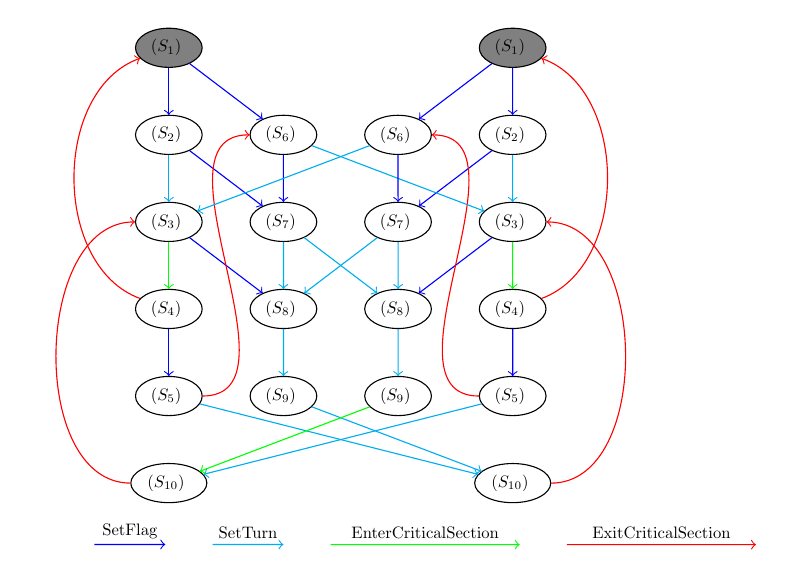
\begin{tikzpicture} [every text node part/.style={align=center},scale=0.6, transform shape]
		
		\node[ellipse, draw, fill=gray] (s1) {\pa $(S_1)$ };
		\node[ellipse, draw] (s2) [below = of s1] {\pa $(S_2)$ };
		\node[ellipse, draw] (s3) [below = of s2] {\pa $(S_3)$ };
		\node[ellipse, draw] (s4) [below = of s3] {\pa $(S_4)$ };
		\node[ellipse, draw] (s5) [below = of s4] {\pa $(S_5)$ };
		
		\node[ellipse, draw] (s6) [right = of s2] {\pa $(S_6)$ };
		\node[ellipse, draw] (s7) [below = of s6] {\pa $(S_7)$ };
		\node[ellipse, draw] (s8) [below = of s7] {\pa $(S_8)$ };
		\node[ellipse, draw] (s9) [below = of s8] {\pa $(S_9)$ };
		
		
		\node[ellipse, draw] (q6) [right = of s6] {\pb $(S_6)$ };
		\node[ellipse, draw] (q7) [below = of q6] {\pb $(S_7)$ };
		\node[ellipse, draw] (q8) [below = of q7] {\pb $(S_8)$ };
		\node[ellipse, draw] (q9) [below = of q8] {\pb $(S_9)$ };
		
		
		\node[ellipse, draw] (q2) [right = of q6] {\pb $(S_2)$ };
		\node[ellipse, draw,fill=gray] (q1) [above= of q2]{\pb $(S_1)$ };
		\node[ellipse, draw] (q3) [below = of q2] {\pb $(S_3)$ };
		\node[ellipse, draw] (q4) [below = of q3] {\pb $(S_4)$ };
		\node[ellipse, draw] (q5) [below = of q4] {\pb $(S_5)$ };
		
		
		\node[ellipse, draw] (q10) [below = of s5] {\pb $(S_{10})$ };
		\node[ellipse, draw] (s10) [below = of q5] {\pa $(S_{10})$ };
		
		\coordinate[below left = of q10] (c1);
		\coordinate[right = 1.5cm of c1] (d1);
		\coordinate[right = 1cm of d1] (c2);
		\coordinate[right =1.5cm  of c2] (d2);
		\coordinate[right = of d2] (c3);
		\coordinate[right =4cm of c3] (d3);
		\coordinate[right = of d3] (c4);
		\coordinate[right = 4cm of c4] (d4);
		
		\draw [->,blue,text=black] (c1) to node[auto]{SetFlag} (d1);
		\draw [->,cyan,text=black] (c2) to node[auto]{SetTurn} (d2);
		\draw [->,green,text=black] (c3) to node[auto]{EnterCriticalSection} (d3);
		\draw [->,red,text=black] (c4) to node[auto]{ExitCriticalSection} (d4);
		
		\path[->]
		(s1) edge [blue] (s2)
		(s1) edge [blue] (s6)
		(q1) edge [blue] (q2)
		(q1) edge [blue] (q6)
		(s2) edge [cyan] (s3)
		(s2) edge [blue] (s7)
		(q2) edge [cyan] (q3)
		(q2) edge [blue] (q7)
		(s3) edge [green] (s4)
		(s3) edge [blue] (s8)
		(q3) edge [green] (q4)
		(q3) edge [blue] (q8)
		(s4) edge [blue] (s5)
		(q4) edge [blue] (q5)
		(s4) edge [red ,bend left=70] (s1)
		(q4) edge [red, bend right=70] (q1)
		(s5) edge [red,out=0,in=180] (s6)
		(s5) edge [cyan] (s10)
		(q5) edge [red,out=180,in=0] (q6)
		(q5) edge [cyan] (q10)
		
		(s6) edge [cyan] (q3)
		(s6) edge [blue] (s7)
		(q6) edge [cyan] (s3)
		(q6) edge [blue](q7)
		(s7) edge[cyan] (q8)
		(s7) edge[cyan] (s8)
		(q7) edge[cyan] (s8)
		(q7) edge[cyan] (q8)
		(s8) edge[cyan] (s9)
		(q8) edge [cyan](q9)
		(s9) edge [cyan](s10)
		(q9) edge[green] (q10)
		(s10) edge[out=0,in=0,red] (q3)
		(q10) edge[out=180,in=180,red] (s3)
		;
		
	\end{tikzpicture}
\end{frame}
\section{\tla Proof System Architecture}

\begin{frame}
	\frametitle{\tla Proof System Architecture}
	\begin{figure}[h]
		\resizebox{\linewidth}{0.7\textheight}{
		\pgfdeclarelayer{background}
		\pgfdeclarelayer{foreground}
		\pgfsetlayers{background,main,foreground}
		
		% Define block styles used later
		
		\tikzstyle{box}=[draw, fill=white!20, text width=12em, 
		text centered, minimum height=3em,drop shadow]
		
		
		\tikzstyle{solver}=[draw, fill=white!20, text width=6em, 
		text centered, minimum height=2em,drop shadow]
		
		
		\tikzstyle{ide}=[draw, fill=green!20, text width=5em, 
		text centered, minimum height=12em,drop shadow]
		
		% Define distances for bordering
		\def\blockdist{2.3}
		\def\edgedist{2.5}
		
		\begin{tikzpicture}
			
			\node (box) [box] {interpret proofs \\ compute proof obligations};
			\path (box.east)+(8em,0) node (box1) [box] {coalesce modal /first-order expressions};
			\path (box1.south)+(0,-3em) node (box2) [box] {call backend provers to attempt proof};
			\path (box.south)+(0,-3em) node (box3) [box] {certify proof \\ (optional, when possible)};
			
			\path (box.north)+(-1,1em) node (box0) {Proof manager};
			
			\path [draw, -> ] (box.east) -- node [above] {} (box1.west);
			\path [draw, -> ] (box1.south) -- node [above] {} (box2.north);
			\path [draw, -> ] (box2.west) -- node [above] {} (box3.east);
			
			
			
			\path (box3.south)+(-2,-4em) node (box4) [solver] {SMT Solvers};
			\path (box4.east)+(4em,0) node (box5) [solver] {Zenon};
			\path (box5.east)+(4em,0) node (box6) [solver] {Isabelle};
			\path (box6.east)+(4em,0) node (box7) [solver] {PTL (Is4)};
			\path (box7.east)+(1.5em,0) node (box8) {...};
			
			\path [draw, <-> ] (box4.north) -- node [above] {} (box2.south);
			\path [draw, <-> ] (box5.north) -- node [above] {} (box2.south);
			\path [draw, <-> ] (box6.north) -- node [above] {} (box2.south);
			\path [draw, <-> ] (box7.north) -- node [above] {} (box2.south);
			
			\begin{pgfonlayer}{background}
				\path (box0.west |- box0.north)+(-4em,3em) node (a) {};
				\path (box8.south -| box8.east)+ (2em,-2em) node (c) {};
				
				\path[fill=orange!20,rounded corners, draw=black!50, thick]
				(a) rectangle (c);           
			\end{pgfonlayer}
			\begin{pgfonlayer}{background}
				\path (box.west |- box.north)+(-2em,2em) node (a) {};
				\path (box2.south -| box2.east)+ (2em,-2em) node (c) {};
				
				\path[fill=blue!20,rounded corners, draw=black!50, thick]
				(a) rectangle (c);           
			\end{pgfonlayer}
			
			\path (box0.north)+(-1,1em) node (boxa) {\tla Proof System};
			
			
			\path (boxa.west)+(-6em,-6em) node (ide) [ide] {\tla \\ Toolbox};
			
			\path [draw, -> ] (ide.30) -- node [above] {} (box.west);
			\path [draw, -> ] (box3.west) -- node [above] {} (ide.315);
			
		\end{tikzpicture}
}
	\end{figure}
\end{frame}

\section{Proving Mutual Exclusion for Peterson's Algorithm in \tla}

\begin{frame}
	\frametitle{Proving Mutual Exclusion for Peterson's Algorithm in \tla}
	\framesubtitle{Proof Structure}
	\begin{itemize}
		\item Structured as an \textbf{Invariance Proof}
		\item For every state in the system, prove that the invariant holds
		\item Use the invariant to prove that the desired property (here, mutual exclusion) holds for the system
	\end{itemize}
\end{frame}

\begin{frame}
	\frametitle{Proving Mutual Exclusion for Peterson's Algorithm in \tla}
	\framesubtitle{Proof Outline}
	\begin{itemize}
		\item Begin by proving that in the initial state, the invariant\footnotemark\   holds
		\item Iterate through every possible state in the system and prove that the invariant holds in that state
		\item For every intermediate state of the system, prove that a state change does not violate the invariant
		\item Prove that the invariant implies mutual exclusion and thereby by a transitive relation, the system also implies mutual exclusion
	\end{itemize}

\footnotetext[2]{$Inv \triangleq ExecutionInvariant \AND TypeInvariant$}
\end{frame}

\begin{frame}
	\frametitle{Proving Mutual Exclusion for Peterson's Algorithm in \tla}
	\framesubtitle{Proof specification in \tla : Initial state}
	
	\fontsize{8}{7.2}\selectfont
	$\THEOREM Spec \implies \square MutualExclusion$\\
	$\PROOF$\\
	\hspace*{0.8cm}$\langle1\rangle1. Init \implies Inv$\\
	\hspace*{1.2cm} $\BY \DEFS Init, Inv, TypeInvariant, ExecutionInvariant, vars,States,ProcSet$\\~\\
	\begin{block}{Proof Decomposition}
		$ Init \triangleq flag = [i \in ProcSet \mapsto \FALSE]$ \\
		\hspace*{0.8cm}$\AND turn \in \{0,1\}$\\
		\hspace*{0.8cm}$\AND  state =  [i \in ProcSet \mapsto "Start"]$\\~\\ 
		$ ExecutionInvariant \triangleq \forall i \in ProcSet:"$ \\
		\hspace*{0.8cm}$state[i] \in States \setminus  \{"Start"\} \implies flag[i] $\\
		\hspace*{0.8cm}$\AND  state[i] \in \{"CriticalSection"\} \implies state[Not(i)] \notin \{"CriticalSection"\}$\\
		\hspace*{0.8cm}$\AND state[Not(i)] \in \{"Waiting"\} \implies turn = i$\\~\\
		$ TypeInvariant \triangleq state \in [ProcSet \rightarrow States]$ \\
		\hspace*{0.8cm}$\AND turn \in ProcSet$\\
		\hspace*{0.8cm}$\AND flag \in [ProcSet \rightarrow \{true, false\}]$
	\end{block}

\end{frame}
\begin{frame}
		\frametitle{Proving Mutual Exclusion for Peterson's Algorithm in \tla}
	\framesubtitle{Proof specification in \tla : Initial state}
	
	\fontsize{8}{7.2}\selectfont
	$\THEOREM Spec \implies \square MutualExclusion$\\
	$\PROOF$\\
	\hspace*{0.8cm}$\langle1\rangle1. Init \implies Inv$\\
	\hspace*{1.2cm} $\BY \DEFS Init, Inv, TypeInvariant, ExecutionInvariant, vars,States,ProcSet$\\~\\
	\begin{block}{Proof Decomposition}
		$ Init \triangleq flag = [i \in ProcSet \mapsto \FALSE]$ \\
		\hspace*{0.8cm}$\AND turn \in \{0,1\}$\\
		\hspace*{0.8cm}$\AND  state =  [i \in ProcSet \mapsto "Start"]$\\~\\ 
		Using the definition of $Init$ we can expand the Invariants. Since both processes have their state set to $"Start"$ and their $flag$ set to $\FALSE$, we can replace the values in the $ExecutionInvariant$ to get: \\~\\
		$ ExecutionInvariant \triangleq \forall i \in ProcSet:"$ \\
		\hspace*{0.8cm}$"Start" \in States \setminus  \{"Start"\} \implies \FALSE $\\
		\hspace*{0.8cm}$\AND  "Start" \in \{"CriticalSection"\} \implies "Start" \notin \{"CriticalSection"\}$\\
		\hspace*{0.8cm}$\AND "Start" \in \{"Waiting"\} \implies turn = i$\\~\\
		$ TypeInvariant \triangleq state \in [ProcSet \rightarrow States]$ \\
		\hspace*{0.8cm}$\AND turn \in ProcSet$\\
		\hspace*{0.8cm}$\AND flag \in [ProcSet \rightarrow \{true, false\}]$
	\end{block}
\end{frame}

\begin{frame}
	\frametitle{Proving Mutual Exclusion for Peterson's Algorithm in \tla}
	\framesubtitle{Proof specification in \tla : Intermediate States}
	\fontsize{8}{7.2}\selectfont
	\hspace*{0cm}$\langle1\rangle2. Inv \AND [Next]_{vars} \implies Inv'$\\
	\hspace*{0.4cm} $\BY \DEFS Init, Inv, TypeInvariant, ExecutionInvariant, vars,States,ProcSet$\\~\\
	\hspace*{0.8cm}$\langle2\rangle1. \SUFFICES \ASSUME Inv,Next\  \PROVE Inv'$\\
	\hspace*{1.2cm} $\BY \DEFS ExecutionInvariant,TypeInvariant,Inv,vars$\\~\\
\end{frame}

\begin{frame}
	\frametitle{Proving Mutual Exclusion for Peterson's Algorithm in \tla}
	\framesubtitle{Proof specification in \tla : Intermediate States contd.}
	\fontsize{8}{10}\selectfont
	
	\hspace*{0cm}$\langle2\rangle2. TypeInvariant'$\\
	\hspace*{0.4cm} $\BY \langle2\rangle1$\\
	\hspace*{0.4cm}$ \DEFS Inv, TypeInvariant, Next, proc, Not, States, ProcSet,$\\
	\hspace*{0.4cm}$ SetFlag, SetTurn, EnterCriticalSection, ExitCriticalSection$\\~\\
\end{frame}

\begin{frame}
	\frametitle{Proving Mutual Exclusion for Peterson's Algorithm in \tla}
	\framesubtitle{Proof specification in \tla : Intermediate States contd.}
	\fontsize{8}{10}\selectfont
	
	\hspace*{0cm}$\langle2\rangle3. ExecutionInvariant'$\\
	\hspace*{0.4cm}$\langle3\rangle1. \SUFFICES \ASSUME \NEW j \in ProcSet\  \PROVE ExecutionInvariant!(j)'$\\
	\hspace*{0.4cm}$\BY \DEFS ExecutionInvariant,ProcSet$\\~\\
	\hspace*{0.4cm}$\langle3\rangle2. \PICK i \in ProcSet : proc(i) $\\
	\hspace*{0.8cm}$\BY \langle2\rangle1 \ \DEFS Next,ProcSet,proc, SetFlag, SetTurn,$\\
	\hspace*{0.8cm}$EnterCriticalSection, ExitCriticalSection$\\~\\
	\hspace*{0.4cm}$\langle3\rangle3. \CASE i =j $\\
	\hspace*{0.8cm}$\BY \langle2\rangle1 , \langle3\rangle2\  \DEFS ExecutionInvariant, TypeInvariant, Inv, proc,$\\
	\hspace*{0.8cm}$Not,ProcSet, SetFlag, SetTurn, EnterCriticalSection, ExitCriticalSection$\\~\\
	\hspace*{0.4cm}$\langle3\rangle3. \CASE i \neq j $\\
	\hspace*{0.8cm}$\BY \langle2\rangle1 , \langle3\rangle2\  \DEFS ExecutionInvariant, TypeInvariant, Inv, proc, Not,ProcSet,$\\
	\hspace*{0.8cm}$SetFlag, SetTurn, EnterCriticalSection, ExitCriticalSection$\\~\\
	\hspace*{0.4cm}$\langle3\rangle. \QED \BY \langle3\rangle3 , \langle3\rangle4 $\\~\\
	\hspace*{0cm}$\langle2\rangle4. \QED \BY \langle2\rangle2 , \langle2\rangle3 \DEF Inv $\\~\\
\end{frame}


\begin{frame}
	\frametitle{Proving Mutual Exclusion for Peterson's Algorithm in \tla}
	\framesubtitle{Proof specification in \tla : Implied Mutual Exclusion}
	\fontsize{8}{10}\selectfont

	\hspace*{0cm}$\langle1\rangle3. Inv \implies MutualExclusion$\\
	\hspace*{0.4cm}$ \BY\DEFS Inv, MutualExclusion,ProcSet,Not,ExecutionInvariant,TypeInvariant$\\~\\
	\hspace*{0cm}$\langle1\rangle4. \QED \BY \langle1\rangle1,\langle1\rangle2,\langle1\rangle3,\langle1\rangle4, \PTL$\\
	\hspace*{0.4cm}$\DEFS MutualExclusion,Spec,ExecutionInvariant, TypeInvariant, Inv, $\\
	\hspace*{0.4cm} $proc, Not,ProcSet, SetFlag, SetTurn, EnterCriticalSection, ExitCriticalSection$\\
	
	\begin{block}{Special Mention}
		PTL is used by the back-end solvers to compute predicates containing Temporal operators. 
	\end{block}
\end{frame}

\begin{frame}
	\frametitle{Proving Mutual Exclusion for Peterson's Algorithm in \tla}
	\framesubtitle{Proof specification in \tla : Toolbox view}
	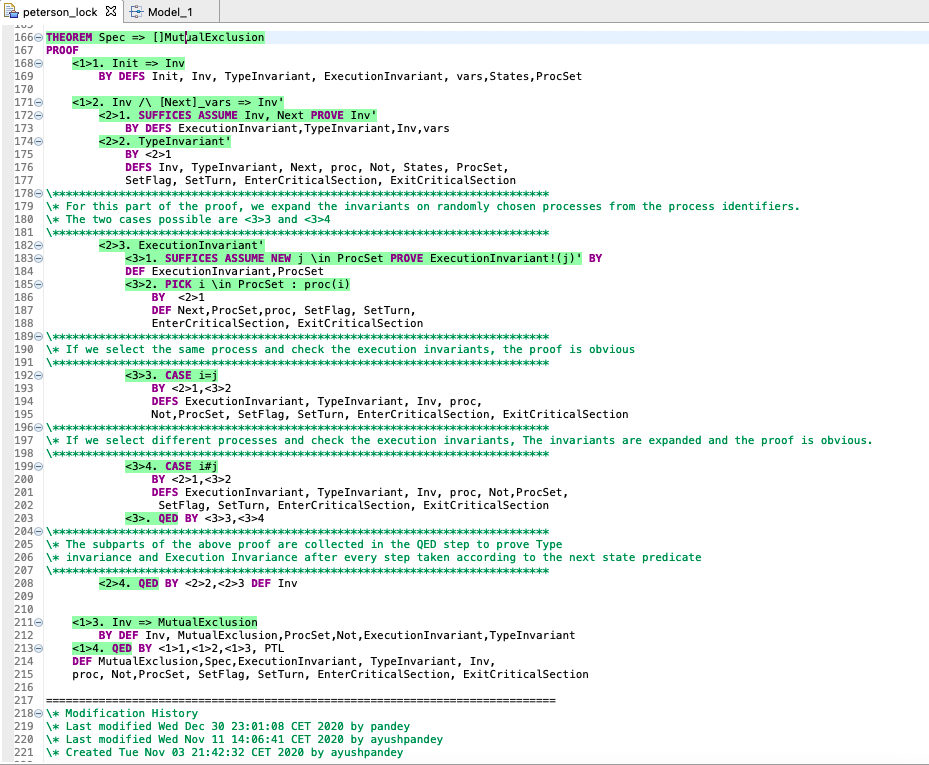
\includegraphics[width=\linewidth,height=\textheight,keepaspectratio]{toolboxproof}
	
\end{frame}

\section{Conclusion}
\begin{frame}
	\frametitle{Conclusion}
	\begin{itemize}
		\item \tla can be used to specify fairly complex systems with ease.
		\item Verification of a specification becomes easier with the mathematical approach.
		\item Several stronger constructs can be used in practice to specify safety, liveness and fairness properties.
		\item Working with \tla requires some experience. It is not straightforward to understand and write a specification for a system.
		\item System specification and proofs can get fairly complex for considerably sized algorithms.
	\end{itemize}
\end{frame}

\begin{frame}
	
\centering
Thank you for your time.\\~\\
Questions??
	
\end{frame}


\begin{frame}
	\nocite{*}
	\bibliographystyle{eptcs}
	\bibliography{references}
\end{frame} 


\begin{frame}
	\frametitle{Appendix: PTL}
	Propositional Temporal Logic (PTL) introduces operators which have specific definitions for interpreting the variables at a given time any instant.\\
	
	\begin{itemize} \scriptsize{
			\item \textbf{$\circ A$}: A holds at the time point immediately after the reference point.\\ (\textit{nexttime operator}).
			
			\item \textbf{$\square A$}: A holds at all time points after the reference point.\\ (\textit{always or henceforth operator}).
			
			\item \textbf{$\diamondsuit A$:} There is a time point after the reference point at which A holds. \\\textit{(sometime or eventually operator)}. 
			
			\item \textbf{$A\  atnext\  B$}: A will hold at the next time point that B holds. \\( \textit{first time or atnext operator}).
			
			\item \textbf{$A\  until\  B$}: A holds at all following time points up to a  time point at which B holds. \\(\textit{until operator}).}
	\end{itemize}
	
	\begin{block}{Remark}
		\tla proof system has a dedicated solver for temporal logic (LS4).
	\end{block}
\end{frame}


\end{document}